\section{低维刚性与弯曲变形}
\label{low:section}
\begin{figure}[htbp]
  \centering
  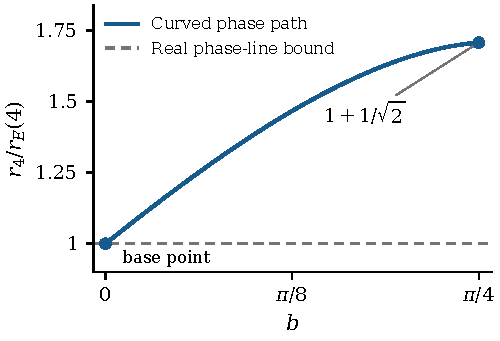
\includegraphics[width=\columnwidth]{figures/fig3_curved.pdf}
  \caption{$n=4$ 时沿显式弯曲相位路径的增强。
  实线由闭式根在 $0\leq b\leq\pi/4$ 上直接计算得到，满足
  $r_4/r_E(4)=\cos[b+\delta(b)]-\sin\delta(b)$，从 $1$ 严格增至 $1+1/\sqrt2$。
  水平虚线表示所有经过指定基点的实相位直线的半径上界。 绘图代码由 OpenAI Codex（GPT-6）辅助编写，并按文中公式核对。}
  \label{fig:curved}
\end{figure}


在固定相位表示中，$n=5$ 这一阈值有一个几何解释。$n=3$ 的指定测量在局部孤立。
$n=4$ 时的规则性方程允许变形，但每一条可行相位直线均不能增加半径；经过同一点的弯曲路径则可以实现增强。

\begin{proposition}[$n=3$ 时的局部刚性]
\label{low:rigidity}
在固定 Pauli 轨道表示中，去除整体相位后，$n=3$ 的指定 EJM 在其相位向量的一个邻域内是孤立的。
\end{proposition}
七个独立相位对应八个带符号局部分量差，其中七个约束的导数在指定点的行列式为
$1/4096$。由逆函数定理，这七个方程的零点局部孤立。
指定点的全部带符号分量均为 $1/4$，故在其邻域内，平方规则性条件与带符号分量相等条件等价。
附录~\ref{low:app-rigidity} 的精确 Jacobian 将文献~\cite{PauwelsGisin2026}
报告的数值秩转化为解析的局部结论。

对于 $n=4$，将任意相位直线写为
\begin{equation}
 M_d(t)=C_4\operatorname{diag}
 \bigl(i^{f_0(z)}e^{itd_z}\bigr)H^{\otimes4},\qquad d_0=0.
 \label{low:line}
\end{equation}
规范 $d_0=0$ 仅去除公共相位，其余 15 个分量可以取任意实数。

图~\ref{fig:curved} 比较相位直线的半径上界与下述弯曲增强。
\begin{theorem}[$n=4$ 时的直线与弯曲增强]
\label{low:theorem}
若直线~\eqref{low:line} 在 $t=0$ 的一个邻域内始终给出共同半径的规则四面体测量，则存在实数 $\omega$ 使
\begin{equation}
 r_d(t)=r_E(4)|\cos(\omega t)|\le r_E(4).
 \label{low:line-bound}
\end{equation}
另一方面，经过同一测量的显式弯曲相位路径满足
\begin{equation}
 r_4\bigl([0,\pi/4]\bigr)
 =\left[r_E(4),\left(1+\frac1{\sqrt2}\right)r_E(4)\right],
 \label{low:curve-range}
\end{equation}
且半径沿该路径严格递增。
\end{theorem}

直线路径的障碍强于 Boolean 模型上界。完整线性化约束核为四维；
二阶条件排除其中一个方向，仅留下一个候选比例，非零三阶项进一步排除该候选。
剩余方向组成两个平面，两者均只产生式~\eqref{low:line-bound} 的余弦规律。
附录~\ref{low:app-lines} 给出明确分类。

为构造能够离开这两个平面的路径，允许两个独立实参数 $b,\delta$，
取式~\eqref{low:masks} 中的两个固定整数掩码 $u,v$，令 $\theta_z=bu_z+\delta v_z$。
在这些相位下，种子的带符号物理 Pauli 分量只有两种取值：十个分量等于 $T/8$，
而 $X_1$ 与 $-Y_4$ 的分量等于 $H/8$，其中
\begin{align}
 T&=\cos(b+\delta)-\sin\delta,\nonumber\\
 H&=\cos b+2\sin\delta\cos b+4\sin b\cos b.
 \label{low:two-components}
\end{align}
这些恒等式在选取路径之前就成立。因此，带符号规则性条件为 $H=T$，
它是关于 $\tan(\delta/2)$ 的二次方程。

经过 $(b,\delta)=(0,0)$ 的根分支具有如下闭式表达。对 $0\le b\le\pi/4$，定义
\begin{align}
 A(b)&=\cos b(1+2\sin b),\nonumber\\
 B(b)&=2\cos b+\sin b+1,\qquad
 C(b)=2\sin b\cos b,\nonumber\\
 \delta(b)&=-2\arctan\frac{2C(b)}
 {B(b)+\sqrt{B(b)^2-4A(b)C(b)}}.
 \label{low:delta}
\end{align}
由此得到相位路径及测量
\begin{equation}
 \begin{aligned}
 \theta_z(b)&=bu_z+\delta(b)v_z,\\
 M_4(b)&=C_4\operatorname{diag}
 \bigl(i^{f_0(z)}e^{i\theta_z(b)}\bigr)H^{\otimes4}.
 \end{aligned}
 \label{low:curve}
\end{equation}
因此，在整条显式路径上，全部带符号分量始终相等。
结合酉性与 Pauli 轨道关系，即得到完整测量及其固定局部四面体。其共同半径为
\begin{equation}
 r_4(b)=r_E(4)\bigl[\cos\bigl(b+\delta(b)\bigr)-\sin\delta(b)\bigr].
 \label{low:curve-radius}
\end{equation}
在闭区间 $0\le b\le\pi/4$ 上，式~\eqref{low:delta} 中根号内的量和分母均严格为正。
附录~\ref{low:app-curve} 证明该分支在此区间内有良好定义，且半径严格递增。
在 $b=0$ 时两个角度均为零，因而逐列恢复原测量。
另一端点满足 $\delta(\pi/4)=-\pi/4$，给出式~\eqref{low:curve-range} 的上端点。
弯曲路径离开可行直线方向组成的两个平面，并满足 $r'_4(0)=\sqrt3/6>0$。

文献~\cite{PauwelsGisin2026} 中另一个 $n=4$ 的测量已经达到更大的半径 $3r_E(4)$。
式~\eqref{low:curve} 的作用是在经过指定 $f_0$ 测量的同时增加半径，并说明为何需要弯曲。
该文所给族的参数段不包含任何在局域酉、比特置换及结果重标号下等价于本指定点的测量。
附录~\ref{low:app-invariant} 使用单比特谱及三个 $2|2$ 划分纯度之和给出简短证书。
更大的规则四面体解流形是否连接这两个族，仍是开放问题。
